\section{Bayesian Experimental Design}

\begin{frame}
  \frametitle{Bayesian experimental design}
  Consider $n$ parameterized experiments:
  $\x_1,\dots,\x_n\in\R^d$.\\
  Each experiment has a real random response $y_i$ such that:
  \begin{align*}
    y_i = \x_i^\top\w^* + \xi_i,\qquad \xi_i\sim\Nc(0,\sigma^2),\quad \Blue{\w^*\sim\Nc(0,\sigma^2\A^{-1})}
  \end{align*}
\textbf{Goal:} Select $k\ll n$ experiments to best estimate $\w^*$
\pause
\begin{columns}
\begin{column}{0.3\textwidth}
\\ \vspace{0.8cm}
Select $S=\{4,6,9\}$\\
\vspace{1cm}
Receive $y_4, y_6, y_9$
\end{column}
\begin{column}{0.5\textwidth}
\begin{center}
	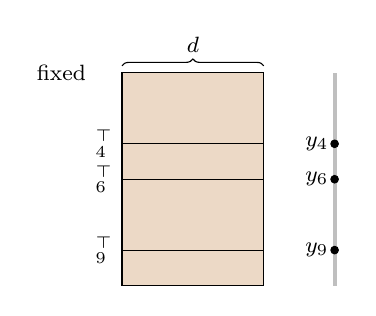
\begin{tikzpicture}[scale=0.9]
          \draw [fill=brown!30] (-2,0) rectangle (0,3);
          \draw [color=black] (-2,2) -- (0,2);
          \draw (-2.25,2) node {\mbox{\footnotesize $\x_4^\top$}}; 
          \draw [color=black] (-2,1.5) -- (0,1.5);
          \draw (-2.25,1.5) node {\mbox{\footnotesize $\x_6^\top$}}; 
          \draw [color=black] (-2,0.5) -- (0,0.5);
          \draw (-2.25,0.5) node {\mbox{\footnotesize $\x_9^\top$}}; 
	   \draw (-2.8,3) node {\footnotesize fixed $\X$}; 
          \draw [decorate,decoration={brace}] (-2,3.1) -- (0,3.1);
          \draw (-1,3.4) node {\mbox{\fontsize{8}{8}\selectfont $d$}}; 
            \draw [color=lightgray,line width =0.5mm] (1,0) -- (1,3);
            \draw [color=lightgray] (0.75,3) node {$\y$};
            \draw (0.75,2) node {\mbox{\footnotesize $y_4$}}; 
            \draw (1,2) node {.}; 
            \draw[mark=*,mark size=1.5pt] plot coordinates{(1,2)};
            \draw (0.75,1.5) node {\mbox{\footnotesize $y_6$}}; 
            \draw (1,1.5) node {.}; 
            \draw[mark=*,mark size=1.5pt] plot coordinates{(1,1.5)};
            \draw (0.75,0.5) node {\mbox{\footnotesize $y_9$}}; 
            \draw[mark=*,mark size=1.5pt] plot coordinates{(1,.5)};
	\end{tikzpicture}
\end{center}
\end{column}
\end{columns}
\end{frame}

\begin{frame}
  \frametitle{Bayesian A-optimal design}
Given the Bayesian assumptions, we have
  \begin{align*}
  \w\mid \y_S \ \sim\ \Nc\Big(\ (\X_S^\top\X_S + \A)^{-1}\X_S^\top\y_S
  ,\ \ \sigma^2(\X_S^\top\X_S+\A)^{-1}\ \Big),
  \end{align*}
  
  Bayesian A-optimality criterion:
\begin{align*}
f_{\A}(\X_S^\top\X_S)=\tr\big((\X_S^\top\X_S+\A)^{-1}\big).
\end{align*}

\textbf{Goal:} Efficiently find subset $S$ of size $k$ such that:
\begin{align*}
f_{\A}(\X_S^\top\X_S)\leq (1+\epsilon)\cdot\underbrace{\min_{S':|S'|=k}f_{\A}(\X_{S'}^\top\X_{S'})}_{\opt}
\end{align*}
\end{frame}

\begin{frame}
  \frametitle{Relaxation to a semi-definite program}
  \begin{block}{SDP relaxation}
The following can be found via an SDP solver in polynomial time:
  \begin{align*}
p^* \ = \  \argmin_{p_1,...,p_n}\ \
  f_{\A}\Big(\sum_{i=1}^np_i\x_i\x_i^\top\Big),\\
\text{subject to}\quad
  \forall_i\ \ 0\leq p_i\leq 1,\quad \sum_i p_i=k.
  \end{align*}
\end{block}

\pause

The solution $p^*$ satisfies $f_{\A}\big(\sum_{i}p_i \x_i \x_i^\top\big)\leq\opt$.

\pause

\textbf{Question:}
For what $k$ can we efficiently round this to $S$ of size $k$?
    
\end{frame}

\begin{frame}
  \frametitle{Efficient rounding for \emph{effective dimension} many
    points\footnote{\tiny\fullcite{bayesian-experimental-design}}}
  \begin{definition}
Define $\A$-effective dimension as $d_{\A} =\tr\big(\X^\top\X(\X^\top\X+\A)^{-1}\big) \leq d$.
\end{definition}
\pause
  \begin{theorem}
If $k=\Omega\big(\frac{d_{\A}}{\epsilon} +
\frac{\log1/\epsilon}{\epsilon^2}\big)$,
then there is a polynomial time 
  algorithm that finds subset $S$ of size $k$ such that
  \begin{align*}
    f_{\A}\big(\X_S^\top\X_S\big) \leq (1+\epsilon)\cdot\opt.
  \end{align*}
\end{theorem}

\pause

\textbf{Remark:} Extends to other Bayesian criteria:
C/D/V-optimality.

\pause

\textbf{Key idea:} \ Sampling $k$-DPP that depends on SDP solution and $\A$

\vspace{5mm}
\end{frame}

\begin{frame}
  \frametitle{Comparison with prior work}
  \centering
    \renewcommand{\arraystretch}{1.5}
\begin{tabular}{r||c|c|l}
 &Criteria&Bayesian&$k=\Omega(\cdot)$\\
  \hline\hline
\small (WYS17) %\cite{tractable-experimental-design}
  &\small A,V&\xmark&$\frac{d^2}{\epsilon}$\\
\small (ALSW17) %\cite{near-optimal-design}
  &\small A,C,D,E,G,V&\cmark&$\frac {d}{\epsilon^2}$\\
\small (NST19) %\cite{proportional-volume-sampling}
  &\small A,D&\xmark&$\frac{d}{\epsilon} +
  \frac{\log1/\epsilon}{\epsilon^2}$\\
  \hline
\small\textbf{our result} (DLM20)%\cite{bayesian-experimental-design}
&\small A,C,D,V&\cmark& $\frac{d_{\A}}{\epsilon} +
  \frac{\log1/\epsilon}{\epsilon^2}$
\end{tabular}
\end{frame}

\begin{frame}{Experiments}
    \begin{figure}
        \centering
        \includegraphics[width=\textwidth]{Figures/design/mg_combined.pdf}
    \end{figure}
\end{frame}